\subsection*{Variable: $CO_2$ Concentration}
The first test is performed with $CO_2$ sensor from the bedroom 1 on the second floor (group 8 and sensor ID 646 in Table 2). The test data is from November 1st, 2012 until February 28th, 2013. One example week from that four month period is shown in Figure~\ref{fig:co2_1}. The classification levels defined in Chapter 4.1 are shown in the figure as well as one missing part that is covered with linear interpolation. For $CO_2$ the minimum level for an alert is set to S2, which is the red line in the picture.

\begin{center}
\begin{figure}[h!]
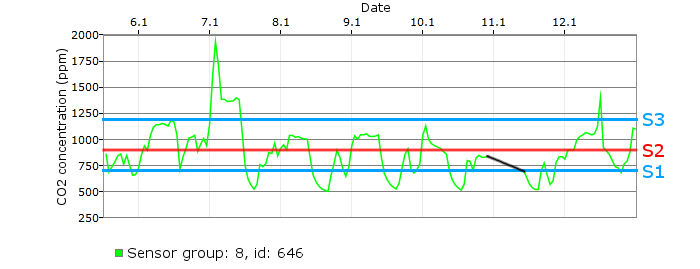
\includegraphics[scale=0.7]{images/co2_1.png}
\caption{Example time series from $CO_2$ sensor. The S1, S2 and S3 mark the classification limits.}
\label{fig:co2_1}
\end{figure}
\end{center}

First, let us investigate the effects of DTW and kNN parameters on the classification results. It is reasonable to suppose that the values of \emph{radius} and \emph{k} should have only a minor effect on the classification results. The time parameters were set to the following values
\begin{itemize}
\item{windowLength: 4 hours}
\item{windowDifference: 1 hour}
\item{waitingInterval: 30 min}
\item{eventInterval: 2 hours}
\item{exceedTime: 30 min}
\end{itemize}

These values mean that a new four-hour predictor vector is created every hour. This predictor is considered positive if the sensor value exceeds the limit value for 30 minutes within two hours after the predictor and a waiting time of 30 minutes.

A 30-day period from November 2012 with a total of 267,524 events was used to test the six parameter combinations. The first 70 \% of the data was used for training and the rest for testing. The classification results are shown in Table~\ref{table:co2_dtwknn_1}.


\begin{table}
  \caption{Results for November 2012 with DTW and kNN model ($W = 0.5$). The definition of ROC distance $AC_d$ is shown in (\ref{eq:acd}). For each row the number of positive samples is $\text{P} = \text{TP} + \text{FN} = 134$ and the number of negative samples is $\text{N} = \text{FP} = \text{TN} = 99$.} 
  \begin{tabular}{ c | c | c | c | c | c | c | c | c | c }
    \hline
   	\textbf{radius} & \textbf{k} & \textbf{TP} & \textbf{FP} & \textbf{TN} & \textbf{FN} & \textbf{TPR} & \textbf{FPR} & \textbf{Accuracy} & $\mathbf{AC_d}$ \\
	\hline
	5 & 3 & 110 & 18 & 81 & 24 & 0.92 & 0.13 & 0.82 & 0.16 \\
	5 & 7 & 103 & 8 & 91 & 31 & 0.77 & 0.060 & 0.83 & 0.17 \\
	5 & 15 & 101 & 9 & 90 & 33 & 0.75 & 0.067 & 0.82 & 0.18 \\
	50 & 3 & 108 & 15 & 84 & 26 & 0.81 & 0.11 & 0.82 & 0.16 \\
	50 & 7 & 102 & 7 & 92 & 32 & 0.76 & 0.052 & 0.83 & 0.17 \\
	50 & 15 & 103 & 6 & 93 & 31 & 0.77 & 0.045 & 0.84 & 0.17 \\
	\hline
  \end{tabular}
  \label{table:co2_dtwknn_1}
\end{table}

As can be seen from the results, the parameters \emph{radius} and \emph{k} do not have much effect on the classifier performance. Thus, the simplest possible model is selected. For the rest of the experiments values $radius = 5$ and $k = 3$ will be used.

Next, we perform the two experiments described in Chapter 4.4.2. The first test trains the model with 14 days of data and then runs tests in batches of 7 days. The second test runs three iterations, each beginning with a training period of 14 days and then three 7-day test batches. The parameters are the same as in the previous test except for the \emph{exceedTime} which is now set to 1 hour.

The results from these experiments are shown in Table~\ref{table:co2_dtwknn_2}. As can be seen from the table, there is no significant difference between constantly updating model and using the the same model for all tests.


\begin{table}
  \caption{DTW and kNN based model. 1: Periodically trained model. 2: Model that is trained only once.} 
  \begin{tabular}{ c | c | c | c | c }
    \hline
   	\textbf{Week} & \textbf{1: Purpose} & \textbf{1: Accuracy} & \textbf{2: Purpose} & \textbf{2: Accuracy} \\
	\hline
	1 & Training & - & Training & - \\
	2 & Training & - & Training & - \\
	3 & Testing & 0.72 & Testing & 0.72 \\
	4 & Testing & 0.81 & Testing & 0.81 \\
	5 & Testing & 0.71 & Testing & 0.71 \\
	6 & Training & - & Testing & 0.75 \\
	7 & Training & - & Testing & 0.86 \\
	8 & Testing & 0.88 & Testing & 0.94 \\
	9 & Testing & 0.91 & Testing & 0.94 \\
	10 & Testing & 0.75 & Testing & 0.75 \\
	11 & Training & - & Testing & 0.84 \\
	12 & Training & - & Testing & 0.86 \\
	13 & Testing & 0.76 & Testing & 0.72 \\
	14 & Testing & 0.81 & Testing & 0.83 \\
	15 & Testing & 0.81 & Testing & 0.84 \\
	\hline
  \end{tabular}
  \label{table:co2_dtwknn_2}
\end{table}

The $CO_2$ consumption seems to be quite easy to predict with this data set because the peaks are quite wide and they occur with constant intervals. The EPN is likely to capture two kinds of complex events: ones that actually precede peaks and ones that are within a peak indicating that the peak will continue.

As of the beginning of April, 2013, the test house was equipped with a mechanical ventilation system which improved the air quality significantly. This change eliminates the periodic increase in $CO_2$ levels we tried to predict in the previous tests. As a comparison, the model was evaluated with four one-week periods from March and April, 2013. These results are shown in Table~\ref{table:co2_dtwknn_3}.

\begin{table}
  \caption{Performance of DTW and kNN based model in the spring of 2013. The mechanical ventilation system was installed in the beginning of April.} 
  \begin{tabular}{ c | c | c | c | c | c | c | c | c | c | c }
    \hline
   	\textbf{Start} & \textbf{End} & \textbf{P} & \textbf{N} & \textbf{TP} & \textbf{FP} & \textbf{TN} & \textbf{FN} & \textbf{TPR} & \textbf{TNR} & \textbf{Accuracy} \\
	\hline
	01.03.13 & 08.03.13 & 42 & 61 & 19 & 1 & 60 & 23 & 0.45 & 0.98 & 0.77 \\
	08.03.13 & 15.03.13 & 17 & 70 & 7 & 1 & 69 & 10 & 0.41 & 0.99 & 0.87 \\
	15.03.13 & 22.03.13 & 11 & 76 & 2 & 2 & 74 & 9 & 0.18 & 0.97 & 0.87 \\
	29.03.13 & 06.04.13 & 32 & 57 & 25 & 0 & 57 & 7 & 0.78 & 1.00 & 0.92 \\
	06.04.13 & 13.04.13 & 2 & 83 & 0 & 3 & 80 & 2 & 0.00 & 0.96 & 0.94 \\
	13.04.13 & 20.04.13 & 2 & 83 & 0 & 2 & 81 & 2 & 0.00 & 0.98 & 0.95 \\
	20.04.13 & 27.04.13 & 2 & 83 & 1 & 1 & 82 & 1 & 0.50 & 0.99 & 0.98 \\
	\hline
  \end{tabular}
  \label{table:co2_dtwknn_3}
\end{table}

As can be seen from the number of positive testing samples in Table~\ref{table:co2_dtwknn_3}, the $CO_2$ levels decreased after the installation of mechanical ventilation system. Or at least the periodic peaks disappeared. The model now struggles with positive sample with \emph{TPR} being much worse than in the previous tests. In the winter the average \emph{TPR} was $0.76$ for the same model.


\subsection*{Variable: VOC}
As a second test variable we are using Volatile Organic Compounds (VOC). The sensor ID is 789 and the group is 7. It is located in a bedroom in the first floor. 

As the last chapter indicated, we would not get much advantage from parameter optimization. Thus, we continue using the same values $k = 3$ and $radius = 5$. A sample week of the data is shown in Figure~\ref{fig:voc_1}.

\begin{center}
\begin{figure}[h!]
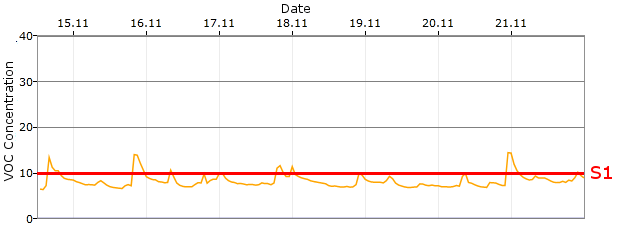
\includegraphics[scale=0.7]{images/voc_1.png}
\caption{VOC concentration.}
\label{fig:voc_1}
\end{figure}
\end{center}

As the figure shows, this time the peaks that exceed the limit value (S1) are much sharper. Thus, we first try to find the optimal time constants. The test data is again from November, 2012.

Two time parameters, \emph{windowDifference} and \emph{exceedTime}, are kept as constants with values 4 hours and 5 min respectively. A small \emph{exceedTime} is required to detect the sharp peaks. The prediction horizon parameters, \emph{windowLength}, \emph{waitingInterval} and \emph{eventInterval} are varied. For each combination a three-fold cross validation is performed and average performances are calculated. The results are shown in Table~\ref{table:voc_dtwknn_1}.

\begin{table}[here]
  \caption{Cross validation performances for DTW and kNN based model with different time parameters and VOC as measurand.} 
  \begin{tabular}{ c | c | c | c | c | c | c }
    \hline
   	\textbf{windowLength} & \textbf{waitingInterval} & \textbf{eventInterval} & \textbf{TPR} & \textbf{FPR} & \textbf{Accuracy} & $\mathbf{AC_d}$ \\
	\hline 
\rowcolor{Good}
2 hours & 30 min & 1  hour & 0.54 & 0.08 & 0.77 & 0.57 \\
\rowcolor{Good}
4 hours &  &  & 0.56 & 0.05 & 0.79 & 0.54 \\
8 hours &  &  & 0.38 & 0.09 & 0.71 & 0.68 \\
2 hours & 1  hour &  & 0.45 & 0.12 & 0.70 & 0.65 \\
\rowcolor{Good}
4 hours &  &  & 0.55 & 0.08 & 0.76 & 0.58 \\
8 hours &  &  & 0.34 & 0.14 & 0.64 & 0.71 \\
2 hours & 2 hours &  & 0.43 & 0.13 & 0.68 & 0.66 \\
4 hours &  &  & 0.48 & 0.07 & 0.73 & 0.62 \\
8 hours &  &  & 0.33 & 0.21 & 0.60 & 0.73 \\
2 hours & 30 min & 2 hours & 0.52 & 0.13 & 0.72 & 0.61 \\
\rowcolor{Good}
4 hours &  &  & 0.55 & 0.09 & 0.75 & 0.58 \\
8 hours &  &  & 0.38 & 0.18 & 0.63 & 0.70 \\
2 hours & 1  hour &  & 0.45 & 0.13 & 0.69 & 0.65 \\
\rowcolor{Good}
4 hours &  & & 0.57 & 0.08 & 0.77 & 0.57 \\
8 hours &  &  & 0.35 & 0.21 & 0.60 & 0.72 \\
2 hours & 2 hours &  & 0.43 & 0.13 & 0.67 & 0.66 \\
4 hours &  &  & 0.50 & 0.14 & 0.70 & 0.63 \\
8 hours &  &  & 0.34 & 0.22 & 0.59 & 0.73 \\
	\hline
  \end{tabular}
  \label{table:voc_dtwknn_1}
\end{table}

The results show that the model misclassifies too many positive samples as negatives. The best parameter combinations are highlighted in the table. Clearly \emph{windowLength} of 4 hours works best. Other two parameters do not show that clear impact so we choose 30 min for \emph{waitingInterval} and 1 hour for \emph{eventInterval} because they produce a simpler model.

The selected model is tested with data starting from the beginning of December 2012. Figure~\ref{fig:voc_dtwknn_test} shows True Positive Rate (\emph{TPR}) and False Positive Rate (\emph{FPR}) for each week.

\begin{center}
\begin{figure}[h!]
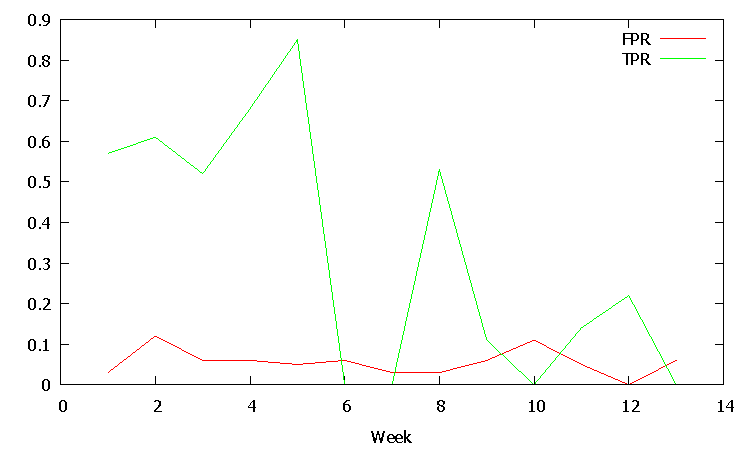
\includegraphics[scale=1.0]{images/voc_dtwknn_test.pdf}
\caption{Weekly \emph{TPR} and \emph{FPR} for DTW and kNN based model starting from the beginning of December 2012.}
\label{fig:voc_dtwknn_test}
\end{figure}
\end{center}

The \emph{FPR} is very small as it was in the parameter selection, too. The \emph{TPR} maintains its level at 0.50-0.60 for five weeks and then drops significantly. Looking at the data shows that the number of limit-exceeding peaks almost disappear in the wintertime. Thus, it is very difficult for the model to predict these rare events.